
%Metadata architecture
% \begin{frame}{Proposed cosmic-ray metadata structure}
%     \vspace{-1.5em}
%     \begin{center}
%         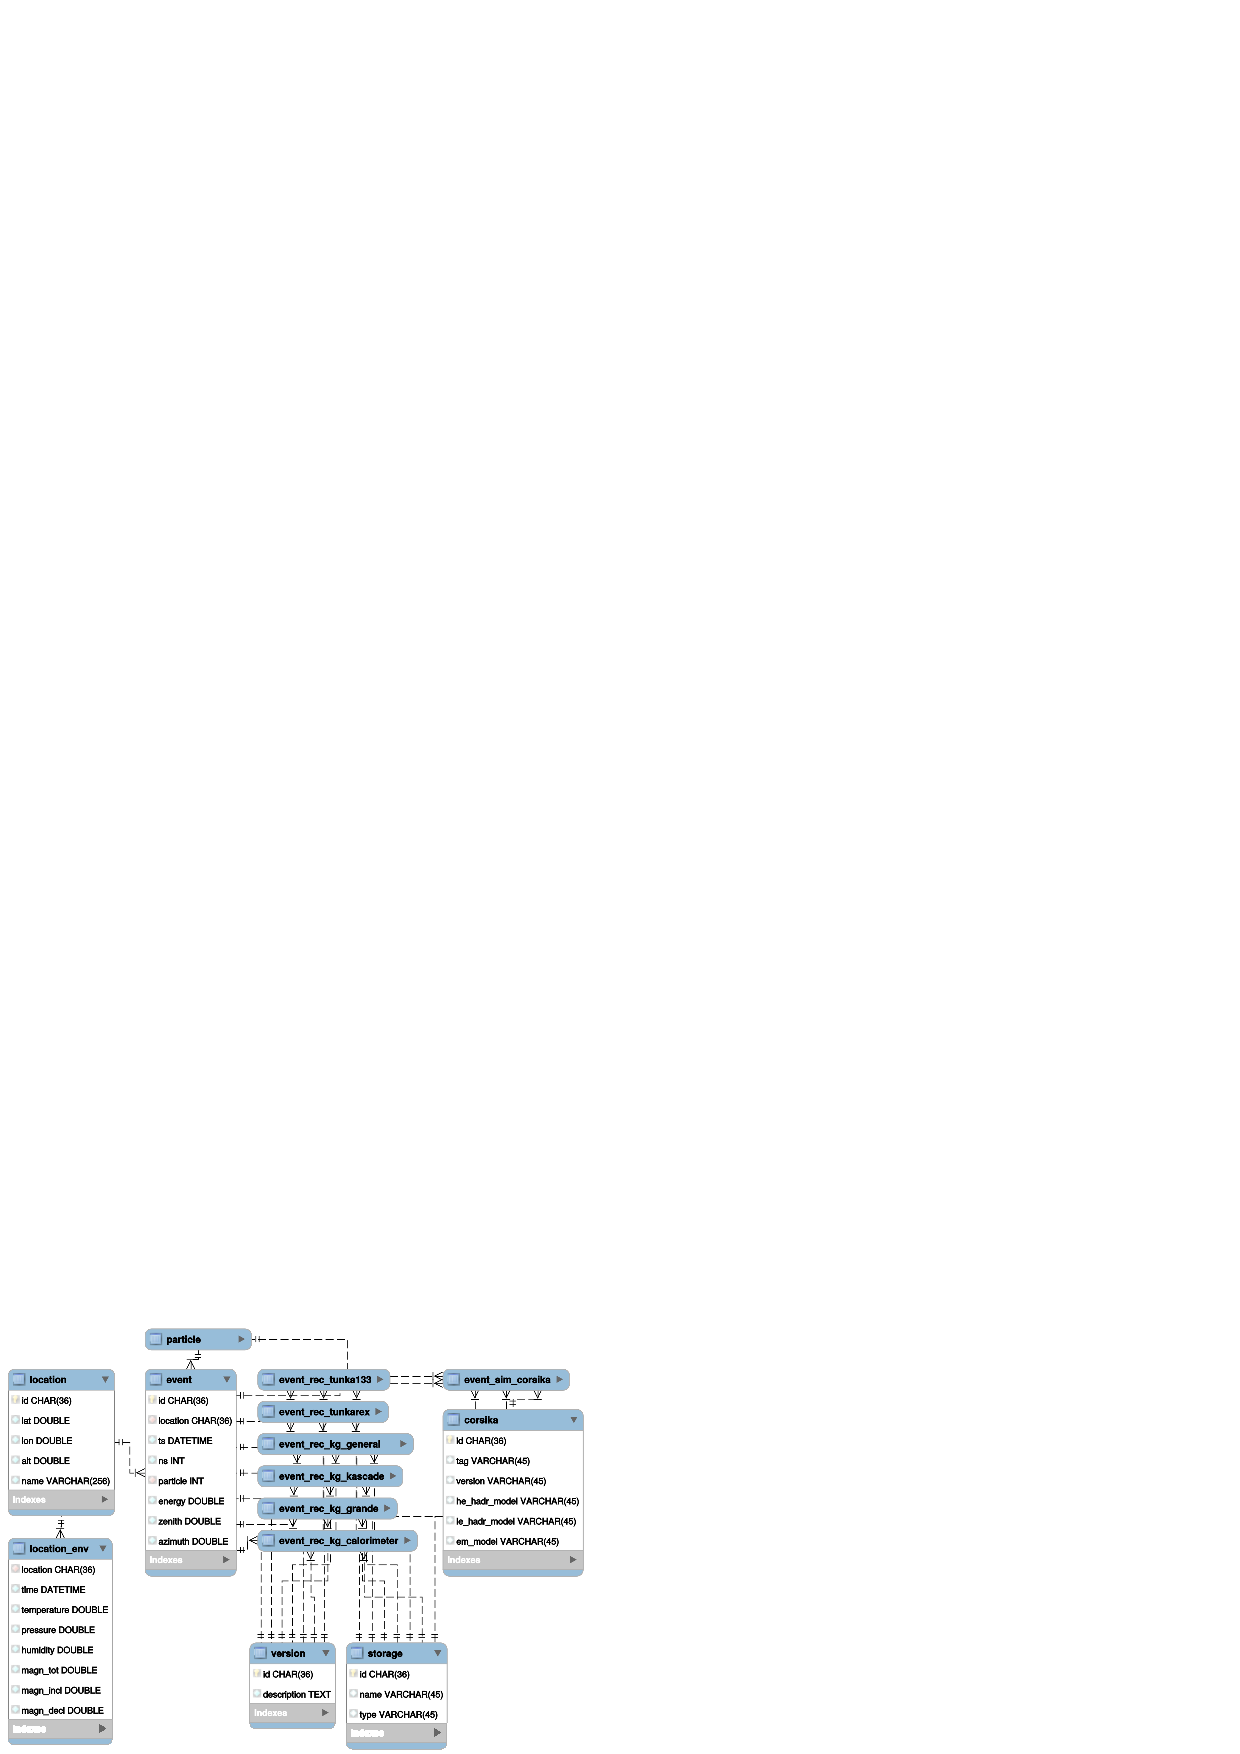
\includegraphics[width=0.82\textwidth]{pics/metadata.pdf}
%     \end{center}
% \end{frame}

\begin{frame}{Aggregation server concept in GRADLC}
\textbf{Aim}: to promote fast reliable access for accumulated data.
\vspace{\itemsep}\\
\textbf{Possible solutions}: CVMFS, PostgreSQL (or TimeScale - ?), TPL.
\vspace{\itemsep}\\
\textbf{Features}:
  \begin{itemize}
    \item Data caching
    \item Fast metadata DB search
  \end{itemize}
\end{frame}

% \begin{frame}{}
%  \begin{item}
%   \item  
%  \end{item}

% \end{frame}

\begin{frame}{Medatata database}
     \begin{center}
        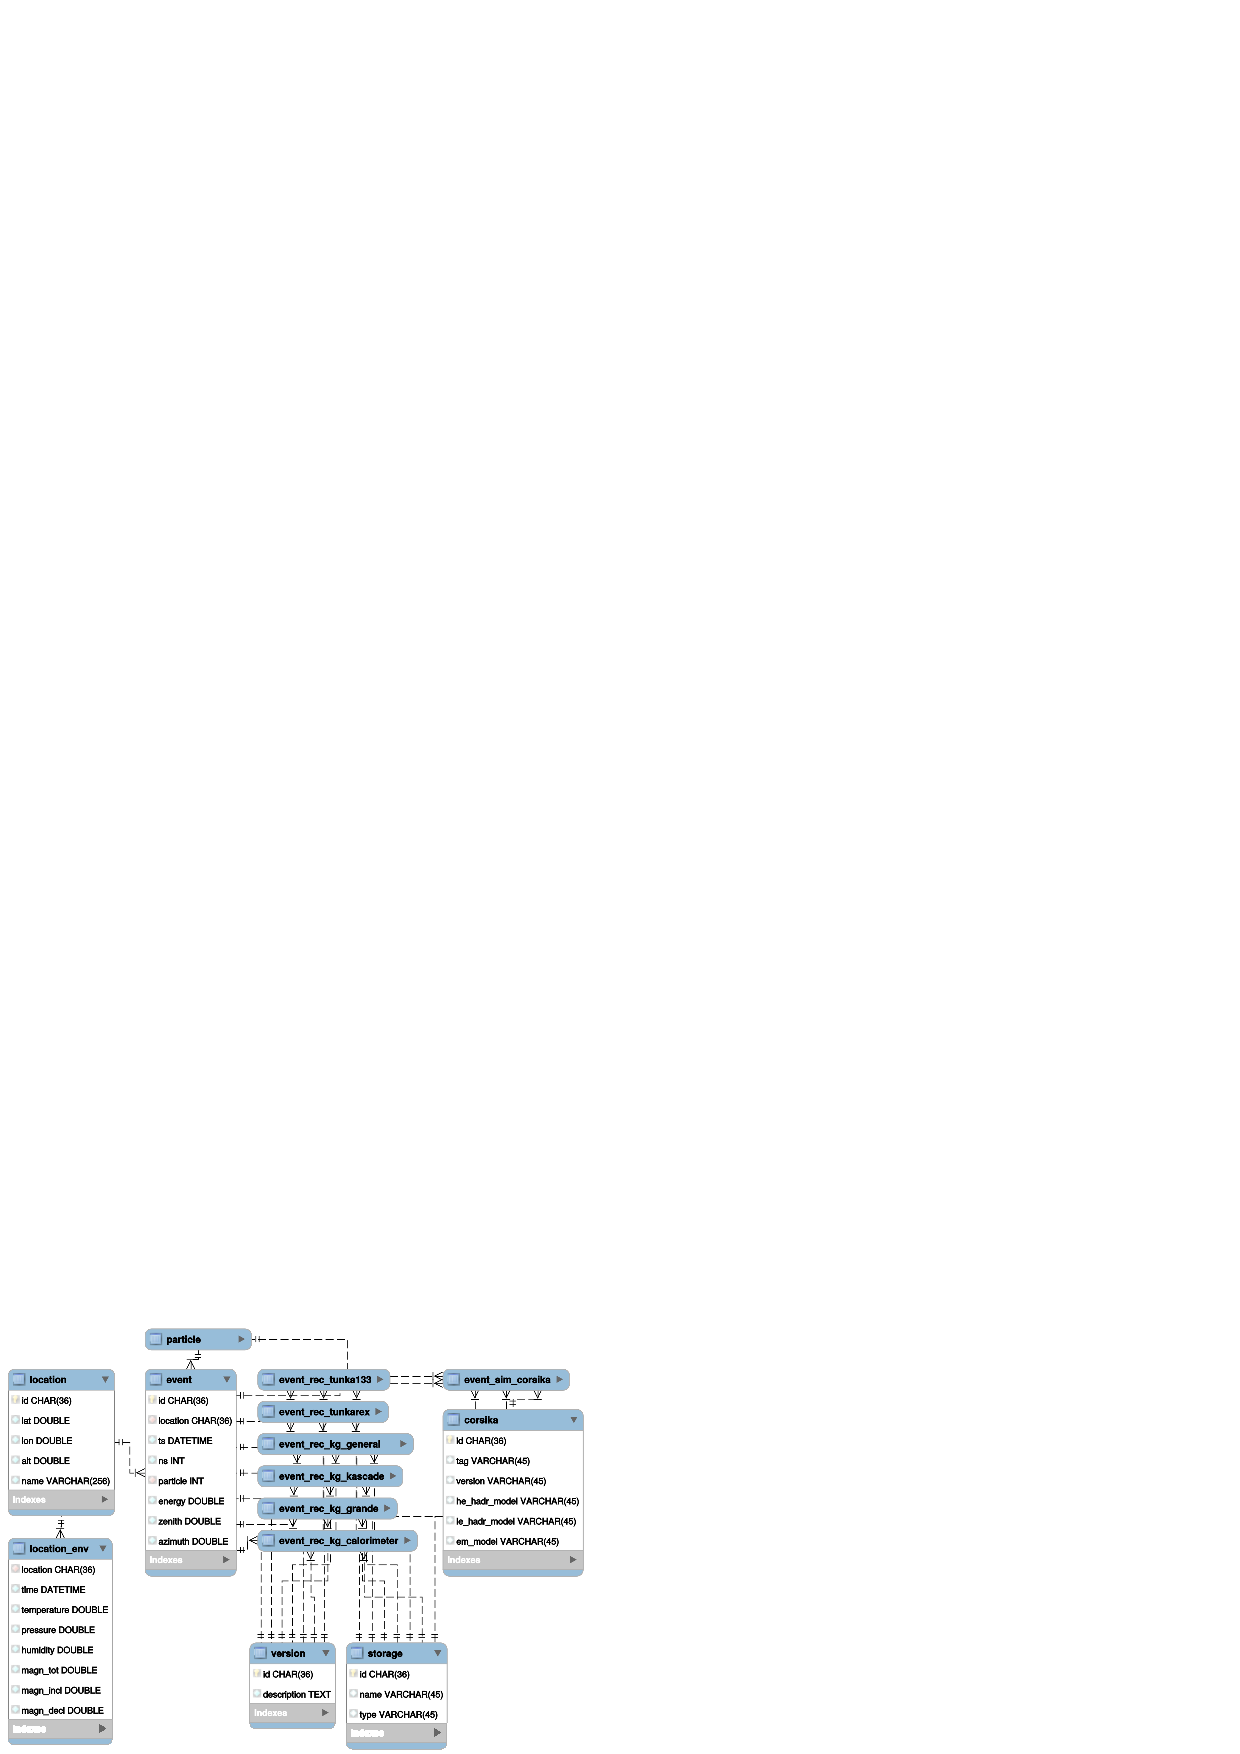
\includegraphics[width=0.82\textwidth]{pics/metadata.pdf}
    \end{center}
\end{frame}

% \begin{frame}{Metadata from the IT point of view}
% 
% Metadata is “data [information] that provides information about other data”
% 
% For example:
% \begin{itemize}
% \item file size
% \item file creation date
% \item file type
% \item file version
% \item release number
% \item reconstruction level
% \end{itemize}
% 
% \end{frame}

% \begin{frame}{Two data access approaches}
% \begin{columns}
%  \begin{column}
%   \begin{itemize}
%    \item 
%   \end{itemize}
% 
%  \end{column}
%   \begin{column}
%     \begin{itemize}
%    \item 
%   \end{itemize}
%  \end{column}
% 
% \end{columns}
% \end{frame}



